% This file is part of the Tractor project.
% Copyright 2012 David W. Hogg (NYU) and Dustin Lang (Princeton).
% All rights reserved.

% to-do
% -----
% - make pickles_to_latex_table.py function
% - make figures showing use of the models in a real situation
% - does the Lupton paper give the profiles, or should we cite the code directly?
% - send to Jim Bosch and Kevin Bundy for comments
% - fix symbols on figures to match text or vice versa (K, M, v, sigma)

\documentclass[12pt,pdftex,preprint]{aastex}
\usepackage{amssymb,amsmath,mathrsfs}

\newlength{\figurewidth}
\setlength{\figurewidth}{0.49\textwidth}

\newcommand{\foreign}[1]{\textit{#1}}
\newcommand{\etal}{\foreign{et\,al.}}
\newcommand{\documentname}{\textsl{Note}}
\newcommand{\project}[1]{\textsl{#1}}
\newcommand{\thetractor}{\project{The~Tractor}}
\newcommand{\sdss}{\project{SDSS}}

\newcommand{\tmatrix}[1]{\boldsymbol{#1}}
\newcommand{\inverse}[1]{{#1}^{-1}}
\newcommand{\transpose}[1]{{#1}^{\mathsf T}}
\newcommand{\tvector}[1]{\boldsymbol{#1}}
\newcommand{\pos}{\tvector{x}}
\newcommand{\spos}{\tvector{\xi}}
\newcommand{\mean}{\tvector{m}}
\newcommand{\var}{\tmatrix{V}}
\newcommand{\affine}{\tmatrix{R}}
\newcommand{\uv}{\tvector{u}}
\newcommand{\zero}{\tmatrix{0}}
\newcommand{\identity}{\tmatrix{I}}
\newcommand{\normal}{N}
\newcommand{\given}{\,|\,}
\renewcommand{\star}{\mathrm{star}}
\newcommand{\dev}{\mathrm{dev}}
\newcommand{\ser}{\mathrm{ser}}
\newcommand{\lux}{\mathrm{lux}}
\newcommand{\luv}{\mathrm{luv}}

\newlength{\figwidth}
\setlength{\figwidth}{0.49\textwidth}

\begin{document}

\title{Replacing standard galaxy profiles with \\ mixtures of Gaussians}
\author{David W. Hogg\altaffilmark{1,2,3} \&
        Dustin Lang\altaffilmark{4}}
\altaffiltext{1}{To whom correspondence should be addressed; \texttt{david.hogg@nyu.edu}}
\altaffiltext{2}{New York University}
\altaffiltext{3}{Max-Planck-Institut f\"ur Astronomie}
\altaffiltext{4}{Princeton University Observatory}

\begin{abstract}
Exponential and de~Vaucouleurs profiles are simple and successful
models for fitting two-dimensional images of galaxies.  One numerical
issue encountered in this kind of fitting is the pixel rendering and
convolution (or correlation) of the models with the telescope
point-spread function (PSF); these operations are slow, and easy to
get slightly wrong at small radii.  Here we exploit the realization
that these models can be approximated to arbitrary accuracy with a
mixture (linear superposition) of two-dimensional Gaussians.  Mixtures
of Gaussians are fast to render and fast to affine-transform.  Most
importantly, if you have a mixture-of-Gaussian PSF model (which we
advocate), the PSF-convolved, affine-transformed galaxy models are
themselves mixtures of Gaussians and therefore very fast to compute
precisely.  We present worked examples that can be directly used in
image fitting; we are using them ourselves.  We discuss extensions to
S\'ersic models and applications of these ideas to three-dimensional
deprojection.
\end{abstract}

Gaussians are remarkable distribution functions.  They have the
incredible properties that---in any number of dimensions---the
convolution (or correlation) of one multivariate Gaussian with another
is itself a multivariate Gaussian, and any product of multivariate
Gaussians is itself a multivariate Gaussian but with a different
normalization.  Furthermore, the means and variance tensors of the
Gaussians output by these operations are related simply to the means
and variance tensors of the inputs.  Add to these wonders the fact
that Gaussians form a complete basis for representing (smooth)
probability distribution functions and it becomes remarkable that we
don't do everything we do in terms of Gaussians.

To elaborate, a mixture of multivariate Gaussians---a linear
superposition---can be used to represent any reasonable distribution
in any number of dimensions to any reasonable precision.  Convolution
(or correlation) by any other distribution that has also been
represented by a mixture of multivariate Gaussians creates a new
mixture of Gaussians with simply adjusted amplitudes, means, and
variance tensors.  The ubiquity of convolution operations in astronomy
suggests the widespread adoption of mixture-of-Gaussian modeling.  We
have pioneered this in the area of distribution modeling in large
numbers of dimensions (\citealt{xd, xdqso, xdqsoz}), where convolution
occurs because the true or noise-free distribution is convolved with
the noise before being observed.  Here we are going to capitalize on
the convolution properties of mixtures of Gaussians in modeling galaxy
morphologies in imaging data, where the true or
high-angular-resolution intensity field is convolved with the
point-spread function (PSF) before being observed.  This is
particularly useful in data sets in which the PSF itself has also been
modeled as a mixture of Gaussians, which is not uncommon (for example,
the \project{Sloan Digital Sky Survey} (\sdss) imaging pipelines
make approximate mixture-of-Gaussian PSF models for
every imaging field; \citealt{lupton}).

We are not the first in this space deconvolution and modeling of
galaxy images with mixtures of Gaussians has been done very
successfully before (for example, \citealt{bendinelli, emsellem,
  bendinelli2, cappellari}).  However, the idea behind those projects
was to use the mixture of Gaussians to provide a very free form for
the isophotes or morphologies of resolved galaxies or other complex
scenes.  Here our goals are very limited: We want to improve the
performance of standard galaxy image model fitting by expressing the
standard galaxy models---the exponential and de~Vaucouleurs
profiles---as rigid mixtures of Gaussians.

The performance advantages we will obtain from using mixtures of
Gaussians are not simply that convolution itself is trivial.  The
standard unconvolved galaxy models, especially the de~Vaucouleurs and
S\'ersic models (\citealt{dev}, \citealt{ser}), are very ill-behaved
near the galaxy center.  Rendering these profiles precisely near the
center can be very challenging numerically.  In addition, most of the
rendering time is spent at very small radii, where PSF convolution is
going to erase all structure anyway.  That is, a mixture-of-Gaussians
description of the de~Vaucouleurs profile saves time both in rendering
\emph{and} in PSF convolution; it produces profiles that are
approximate but very high performance when all real uses of the
profiles are PSF-convolved, as they usually are.

Along those lines, it is important in any image-modeling situation to
think of the PSF as the \emph{pixel-convolved} point-spread function.
Under this choice, synthesis of a pixelized image involves only
convolution with the PSF and sampling at the pixel centers.  That is,
image synthesis (returned to at the end of this \documentname)
consists of PSF convolution (an arithmetic operation on the two
mixtures of Gaussians) followed by sampling (evaluation of the
resulting mixture at the pixel centers).

We need good performance in two-dimensional image synthesis (for
fitting) because, with \thetractor\ (Lang \etal, forthcoming), we are
building a comprehensive model of all the imaging data we have; this
will have models of many millions of galaxies in imaging that contains
on the order of $10^{13}$ pixels.  We are basing our models on the
\sdss\ Catalog galaxy models, which only include exponential,
de~Vaucouleurs, and composite (mixture of the two) radial profiles.
In detail, in fact, the \sdss\ Catalog models are small modifications
of these (\citealt{lupton}); details below.  So our goal here is to
provide replacements for these models in order to improve the
performance of galaxy image modeling and analysis software.  Some of
the models we present have been used previously in tools for precise
photometry (Bundy \etal, forthcoming); they could also be used to
speed other image-fitting systems, like the very successful
\project{GALFIT} (\citealt{galfit}).

Because we are thinking about two-dimensional imaging, we use here
two-dimensional Gaussian or Normal distributions, which look like
\begin{eqnarray}\displaystyle
\normal(\pos\given\mean,\var) &\equiv& \frac{1}{2\pi}\,\det(\var)^{-1/2}\,\exp(-\frac{1}{2}\,\transpose{[\pos-\mean]}\cdot\inverse{\var}\cdot[\pos-\mean])
\quad ,
\end{eqnarray}
where $\pos$ and $\mean$ are two-dimensional vectors (usually in the
focal plane or on the sky or something like that), and $\var$ is a
symmetric $2\times 2$ variance tensor or matrix, and implicitly the
vectors are column vectors.  A \emph{mixture of Gaussians} is a linear
superposition of Gaussians.  Any positive two-dimensional function
with finite support and finite total integral---including as a special
case any two-dimensional probability distribution function---can be
represented as a mixture of Gaussians to arbitrary accuracy; that is
\begin{eqnarray}
p(\pos) &\approx& \sum_{k=1}^K a_k\,\normal(\pos\given\mean_k,\var_k)
\\
1 &=& \sum_{k=1}^K a_k
\quad ,
\end{eqnarray}
where $p(\pos)$ is any probability distribution of a two-dimensional
quantity $\pos$, the $\approx$ symbol implies approximation, $K$ is
the number of Gaussians used in the mixture, and the $K$ Gaussians
have amplitudes $a_k$, means $\mean_k$, and variance tensors $\var_k$.
The sum-to-one condition ensures that the probability distribution
approximation is properly normalized.

We wish to make an approximation to the two-dimensional circular
exponential (exp) profile $Q^{\exp}(\cdot)$
\begin{eqnarray}\displaystyle
Q^{\exp}(\spos) &\equiv& \exp(-\alpha^{\exp}\,[|\spos| - 1])
\\
\alpha^{\exp} &\equiv& 1.67834699
\quad ,
\end{eqnarray}
where $\spos$ is a dimensionless focal-plane position, and
$\alpha^{\exp}$ is a dimensionless inverse length set to ensure that
the profile has unit half-light radius.  The position $\spos$ is
dimensionless because it parameterizes the unit-size dimensionless
function.  We seek the best (where ``best'' will be defined below)
$M^{\exp}$-Gaussian mixture (where $M^{\exp}$ is an integer)
approximation
\begin{eqnarray}\displaystyle
Q^{\exp}(\spos) &\approx& \sum_{m=1}^{M^{\exp}} a^{\exp}_m\,\normal(\spos\given\zero,\var^{\exp}_m)
\\
\var^{\exp}_m &\equiv& v^{\exp}_m\,\identity
\quad ,
\end{eqnarray}
where all of the means are exactly zero and all of the variances
$\var^{\exp}_m$ in the mixture can be represented as a scalar
$v^{\exp}_m$ multiplied by the identity matrix $\identity$
because we are requiring this dimensionless function to be precisely
circular (so every component is itself circular and concentric).
Similarly for the de~Vaucouleurs (dev) profile
\begin{eqnarray}\displaystyle
Q^{\dev}(\spos) &\equiv& \exp(-\alpha^{\dev}\,[|\spos|^{1/4} - 1])
\\
\alpha^{\dev} &\equiv& 7.66924944
\\
Q^{\dev}(\spos) &\approx& \sum_{m=1}^{M^{\dev}} a^{\dev}_m\,\normal(\spos\given\zero,\var^{\dev}_m)
\\
\var^{\dev}_m &\equiv& v^{\dev}_m\,\identity
\quad .
\end{eqnarray}
The half-light inverse-radius parameters $\alpha^{\exp}$ and
$\alpha^{\dev}$ are from \citet{ciotti}.  The challenge we
meet below is to determine the parameters
\begin{eqnarray}
\{a^{\exp}_m,v^{\exp}_m\}_{m=1}^{M^{\exp}}~,~\{a^{\dev}_m,v^{\dev}_m\}_{m=1}^{M^{\dev}}
\end{eqnarray}
to best approximate the traditional galaxy profile functions, under
some sensible definiton of the word ``best'', as a function of the
model complexity parameters (numbers of components) $(M^{\exp},
M^{\dev})$.

In addition to these, there are general S\'ersic (ser) profiles, of
which the exp and dev profiles are special cases.  The general ser
profile has one parameter (the ``index'') $n$:
\begin{eqnarray}\displaystyle
Q^{\ser}(\spos\given n) &\equiv& \exp(-\alpha^{\ser}(n)\,[|\spos|^{1/n} - 1])
\\
\{\alpha^{\ser}(2), \alpha^{\ser}(3), \alpha^{\ser}(5)\} &\equiv& \{3.67206075, 5.67016119, 9.66871461\}
\quad ,
\end{eqnarray}
where we have given the constant $\alpha^{\ser}(n)$ for just a few
values of $n$ (\citealt{ciotti}; the $\exp$ and $\dev$ profiles give
the $n=1$ and $n=4$ values).

The \sdss\ pipelines make use of modified profiles, which have been
truncated smoothly at large radius and (in the case of the
de~Vaucouleurs profile) ``softened'' at the center (\citealt{lupton}).
The \sdss\ form of the exponential (lux) profile is
\begin{eqnarray}\displaystyle
Q^{\lux}(\spos) &\equiv& \left\{\begin{array}{ll}
  \exp(-\alpha^{\lux}\,[|\spos| - 1]) & \mbox{for~}|\spos| < 3 \\
  \exp(-\alpha^{\lux}\,[|\spos| - 1])
  \,\left[1 - [|\spos| - 3]^2\right]^2 & \mbox{for~}3 < |\spos| < 4 \\
  0                                   & \mbox{for~}4 < |\spos|
\end{array}\right.
\\
\alpha^{\lux} &\equiv& 1.67835
\quad ,
\end{eqnarray}
and the \sdss\ form of the de~Vaucouleurs (luv) profile is
\begin{eqnarray}\displaystyle
Q^{\luv}(\spos) &\equiv& \left\{\begin{array}{ll}
  \exp(-\alpha^{\luv}\,\left[[|\spos|^2 + 0.0004]^{1/8} - 1\right]) & \mbox{for~}|\spos| < 7 \\
  \exp(-\alpha^{\luv}\,\left[[|\spos|^2 + 0.0004]^{1/8} - 1\right])
  \,\left[1 - [|\spos| - 7]^2\right]^2 & \mbox{for~}7 < |\spos| < 8 \\
  0                                   & \mbox{for~}8 < |\spos|
\end{array}\right.
\\
\alpha^{\luv} &\equiv& 7.66925
\quad .
\end{eqnarray}
The half-light inverse-radius parameters $\alpha^{\exp}$ and
$\alpha^{\dev}$---and the softening and cutoff radius parameters---are
taken from the \sdss\ codebase.

The profiles above are normalized to have unit intensity
(approximately) at their half-light radii.  In many cases, the
investigator wants profiles that are normalized to have unit total
flux (intensity integrated over solid angle).  Although there is an
analytic result for the dev profile, numerical integration of the
concentrated profiles dev and luv to determine total fluxes can be
challenging.  This is not true for the mixture-of-Gaussian
approximations: Each Gaussian is normalized, so the sum of the
amplitudes $\sum_m a^{\luv}_m$ (for the luv profile, say) gives the
total flux for the mixture-of-Gaussians approximation to that profile.

We seek the \emph{best} mixture-of-Gaussian approximations.  This
necessitates definition of the word ``best''.  If we think of the
profiles as being two-dimensional probability distribution functions
(for, say, the arrivals of photons), then one natural choice is the
K-L divergence or similar cross-entropy or information-theoretic
measure.  However, in typical astronomical imaging, the galaxy is
superimposed on a substantial, flat sky level, and the noise in the
data is close to Gaussian.  This suggests more chi-squared-like
objectives.  We adopt the latter, in part because they are most
appropriate for our specific proposed application (modeling \sdss-like
astronomical imaging), but experiments we have performed suggest that
information-theoretic objectives also lead to good results.

In detail, the chi-squared objective we minimize---the
\emph{badness}---is a squared residual between the exact profile
function $Q(\spos)$ and its mixture-of-Gaussian approximation.  It is
designed to be equivalent to a chi-squared statistic in a
homoskedastic two-dimensional image of the profile taken with
extremely high angular resolution (pixels of size 0.001 the half-light
radius) and vanishing point-spread function.  Quantitatively the
badness is defined to be the mean squared residual in the $Q(\spos)$
functions, which are normalized to have unit intensity at the
half-light radius, averaged over a two-dimensional circular region in
the $\spos$ plane centered on the (circularly symmetric) profile and
extending out to radius $\xi_{\max}$.  We use $\xi_{\max}=8$ for all
profiles except the $\lux$ profile, for which we use $\xi_{\max}=4$.
In practice, the badness is computed in a one-dimensional numerical
integral but the integral is weighted in radius (weight increasing
linearly with radius) to make it equivalent to the two-dimensional
chi-squared.

Optimization (minimization) of the badness is performed by the
\project{scipy} implementation of the BFGS algorithm, with many
initializations to explore multiple local minima.  Further details are
available in the code, which is publicly
available.\footnote{\url{https://github.com/davidwhogg/TheTractor/}}

...Show plots demonstrating quality of fit, one-d and two-d plots...

...give tables of results, including Bundy versions and recommended
versions...Why are we giving and plotting root-variances not
variances?...

...show dependence of amplitudes and variances on sersic n for some
M...be sure to synchronize $\xi_{\max}$...

The value of these mixture-of-Gaussian galaxy components comes when
they are to be convolved with a PSF (usually in fact a pixel-convolved
PSF) that is itself represented as a mixture of Gaussians.  In this
scenario, the PSF $\psi(\Delta\pos)$---which is thought of as a
function of focal-plane displacement $\Delta\pos$ away from, say, a
true stellar position---is represented as a $K$-Gaussian mixture
\begin{eqnarray}\displaystyle
\psi(\Delta\pos) &=& \sum_{k=1}^K p_k\,\normal(\Delta\pos\given\mean_k,\var_k)
\\
1 &=& \sum_{k=1}^K p_k
\quad ,
\end{eqnarray}
where the means $\mean_k$ are \emph{not} required to vanish because
the PSF can have arbitrarily non-trivial structure (think speckles and
the like) and the variances $\var_k$ will not in general be
proportional to the identity or even diagonal because the PSF will not
in general be round.  An example that illustrates the use of this PSF
is the following: A star of flux $S_s$ at focal-plane position
$\pos_s$ will lead to an image (PSF-convolved intensity map) of the
form
\begin{eqnarray}\displaystyle
I(\pos\given\star,S_s,\pos_s) &=& \sum_{k=1}^K S_s\,p_k\,\normal(\pos\given\pos_s+\mean_k,\var_k)
\quad .
\end{eqnarray}
That is, when the PSF is represented as a mixture of Gaussians, any
image of a star---or indeed any image of any set of stars---is also
represented as a mixture of Gaussians.

Applying this PSF to an exp or dev galaxy is slightly more
complicated, because the galaxy has not just a flux $S_g$ and a
central position $\pos_g$; it also has a shape.  Because we are only
considering these simple galaxies, we are only permitting ellipsoidal
shapes, which can be represented by a semi-major axis $a$, a
semi-minor axis $b$, and a position angle $\phi$, or equivalently by
eigenvalues $a, b$ and eigenvectors $\uv_1, \uv_2$, or equivalently by
an affine transformation $\affine_g$ that takes a circle to the
relevant ellipse (and is a therefore a general representation of an
ellipse; it is also the matrix square root of the symmetric variance
tensor describing the ellipse).  The galaxy is distorted by this
affine transformation \emph{prior} to PSF convolution, so the
focal-plane image (PSF-convolved intensity field) for a general (say)
$\exp$ galaxy is given by
\begin{eqnarray}\displaystyle
I(\pos\given\exp,S_g,\pos_g,\affine_g) &=& \sum_{k=1}^K \sum_{m=1}^{M^{\exp}} S_g\,a^{\exp}_m\,p_k\,\normal(\pos\given\pos_g+\mean_k,\var_{gm}+\var_k)
\\
\var_{gm} &\equiv& \affine_g\cdot\var^{\exp}_m\cdot\transpose{\affine_g}
\\
\affine_g &=& \left[a\,\uv_1 , b\,\uv_2 \right]
\quad ,
\end{eqnarray}
where $a$ and $b$ are the major and minor axis lengths of the galaxy
ellipse (in appropriate units) and $\uv_1$ and $\uv_2$ are the
eigenvectors on the sky pointing in the major-axis and minor-axis
directions respectively.  Implicitly all vectors are two-dimensional
column vectors, and $\affine_g$ is a $2\times 2$ affine transformation
matrix that contains the ``shape'' (position angle, major-axis, and
ellipticity) information about the galaxy.  The $\dev$, $\luv$, and
$\lux$ cases are all similar.  Note the important and key result of
this \documentname, to wit, that a mixture-of-Gaussian galaxy model
(with $M$ components) convolved with a mixture-of-Gaussian PSF model
(with $K$ components) yields a mixture-of-Gaussian image (with
$[M\,K]$ components).

...pegagogical figure demonstrating these operations and their results...

...what about mixtures of exps and devs:  No problem!...

\acknowledgements It is a pleasure to thank
      Brendon Brewer (Auckland)
  and Kevin Bundy (IPMU)
for valuable comments.  This work was supported in part by NASA (grant
NNX12AI50G) and the NSF (grant IIS-1124794).

\begin{thebibliography}{70}
\bibitem[Bendinelli(1991)]{bendinelli}
Bendinelli,~O., 1991, \apj, 366, 599
\bibitem[Bendinelli \& Parmeggiani(1995)]{bendinelli2}
Bendinelli,~O. \& Parmeggiani,~G., 1995, \aj, 109, 572
\bibitem[Bovy \etal(2011a)]{xd}
Bovy,~J., Hogg,~D.~W., \& Roweis,~S., 2011, Ann. Appl. Stat., 5, 1657
\bibitem[Bovy \etal(2011b)]{xdqso}
Bovy,~J., \etal, 2011, \apj, 729, 141
\bibitem[Bovy \etal(2012)]{xdqsoz}
Bovy,~J. \etal, 2012, \aj, 749, 41
\bibitem[Cappellari(2002)]{cappellari}
Cappellari,~M., 2002, \mnras, 333, 400
\bibitem[Ciotti \& Bertin(1999)]{ciotti}
Ciotti,~L. \& Bertin,~G., 1999, \aa, 352, 447
\bibitem[de~Vaucouleurs(19xx)]{dev}
de~Vaucouleurs,~G., 19xx, whatever
\bibitem[Emsellem \etal(1994)]{emsellem}
Emsellem,~E., Monnet,~G., Bacon,~R., \& Nieto,~J.-L., 1994, \aap, 285, 739
\bibitem[Lupton \etal(2001)]{lupton}
Lupton,~R., Gunn,~J.~E., Ivezic,~Z., Knapp,~G.~R., Kent,~S.~M., \& Yasuda,~N., 2001, ASPC, 238, 269
\bibitem[Peng \etal(2002)]{galfit}
Peng,~C.~Y., Ho, L.~C., Impey,~C.~D., \& Rix,~H.-W., 2002, \aj, 124, 266
\bibitem[S\'ersic(19xx)]{ser}
S\'ersic,~X., 19xx, whatever
\end{thebibliography}

\clearpage
\begin{table}
\caption{The amplitudes and root-variances for the best
  mixture-of-Gaussian approximations to the various profiles, for
  different mixture sizes.  The badness and total (dimensionless) flux
  are given for each approximation.}
\end{table}

\clearpage
\begin{figure}
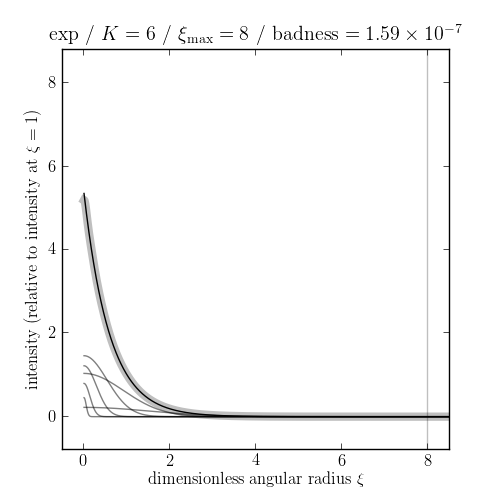
\includegraphics[width=\figurewidth]{exp_K06_MR08_profile.png}%
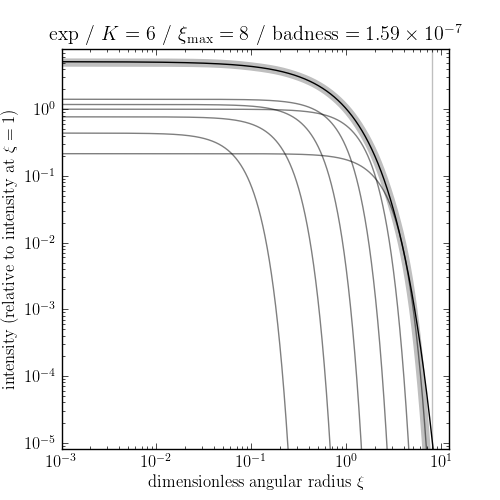
\includegraphics[width=\figurewidth]{exp_K06_MR08_profile_log.png}\\
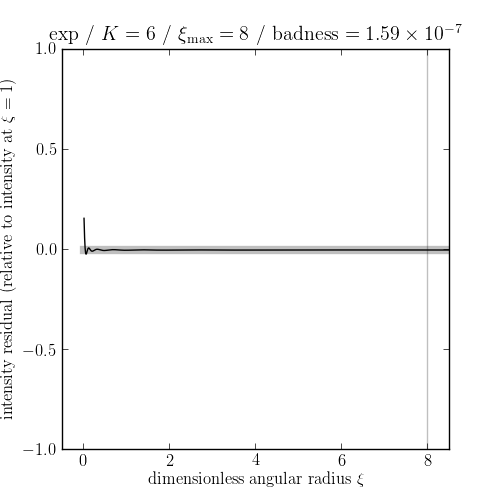
\includegraphics[width=\figurewidth]{exp_K06_MR08_residual.png}%
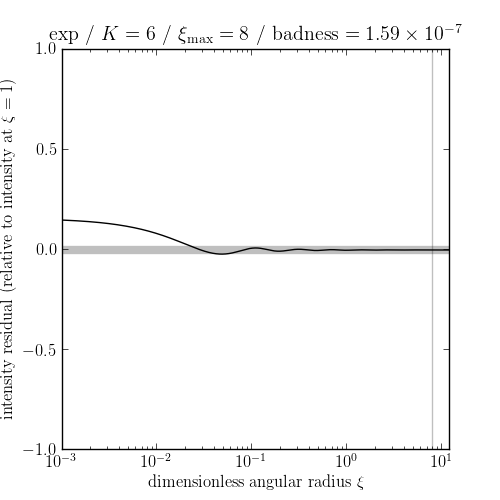
\includegraphics[width=\figurewidth]{exp_K06_MR08_residual_log.png}
\caption{\textsl{top-left:} The true exp profile (thin black line),
  the best $M^{\exp}=6$ mixture-of-Gaussian approximation (thick grey
  line), and the component Gaussians (multiplied by their
  corresponding amplitudes) contributing to the approximation (thin
  grey lines).  The plot title text gives $\xi_{\max}$ and the
  badness. \textsl{top-right:} The same but shown logarithmically.
  \textsl{bottom-left:} A representation of the residual or devation,
  on which the badness is computed.  \textsl{bottom-right:} The same
  but shown logarithmically.\label{fig:exp}}
\end{figure}

\clearpage
\begin{figure}
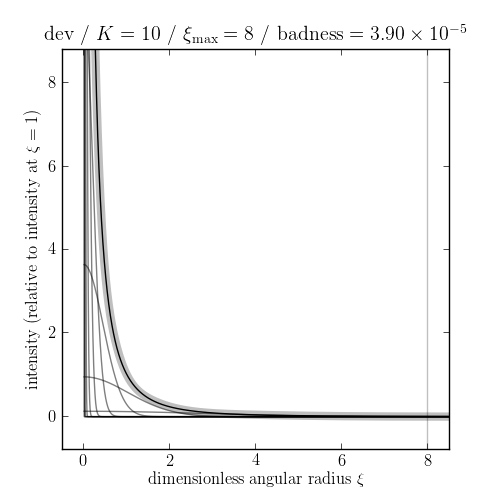
\includegraphics[width=\figurewidth]{dev_K10_MR08_profile.png}%
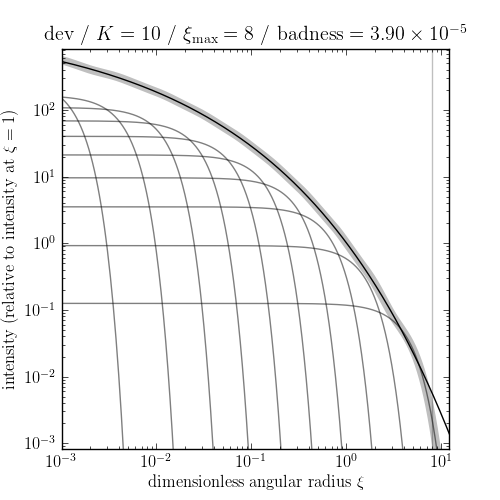
\includegraphics[width=\figurewidth]{dev_K10_MR08_profile_log.png}\\
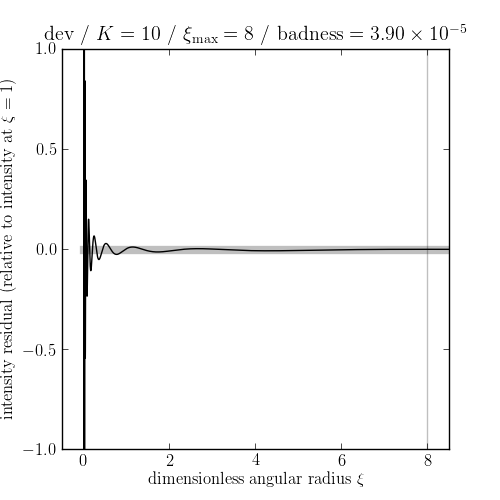
\includegraphics[width=\figurewidth]{dev_K10_MR08_residual.png}%
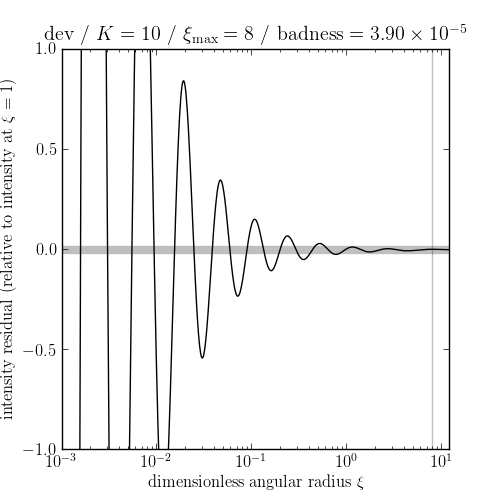
\includegraphics[width=\figurewidth]{dev_K10_MR08_residual_log.png}
\caption{The dev profile and the best $M^{\dev}=10$ approximation.
  The panels are equivalent to those in \figurename~\ref{fig:exp}.
  The residuals look bad in the logarithmic plot, but they are only
  bad very near the profile center (as expected), where the effect of
  any realistic point-spread function will average them away.}
\end{figure}

\clearpage
\begin{figure}
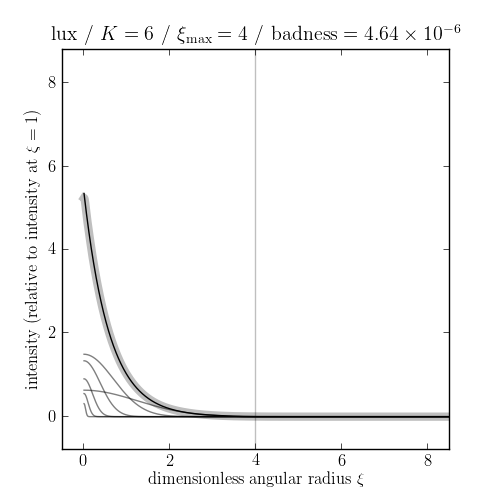
\includegraphics[width=\figurewidth]{lux_K06_MR04_profile.png}%
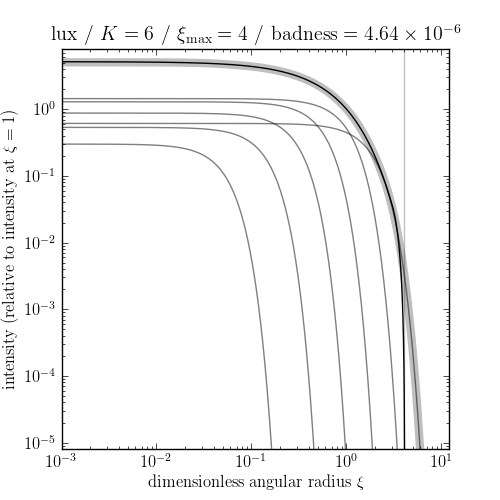
\includegraphics[width=\figurewidth]{lux_K06_MR04_profile_log.png}\\
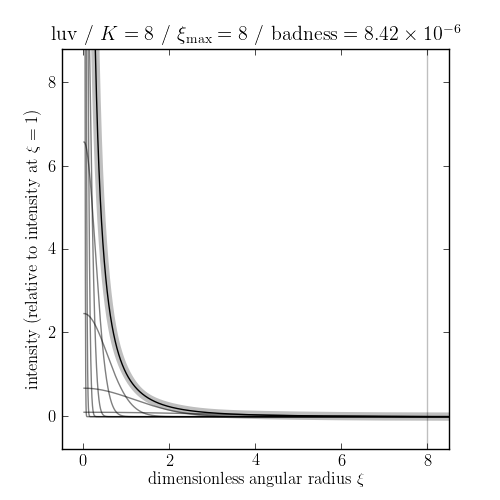
\includegraphics[width=\figurewidth]{luv_K08_MR08_profile.png}%
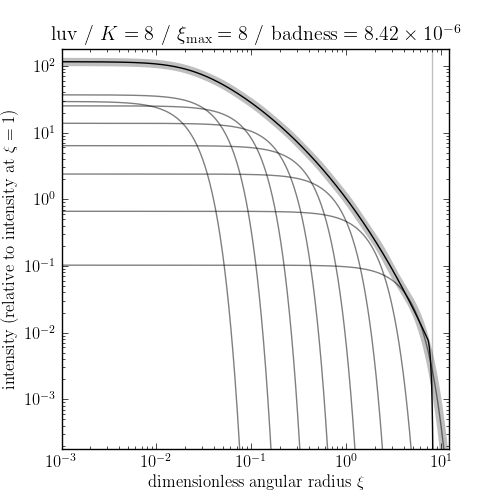
\includegraphics[width=\figurewidth]{luv_K08_MR08_profile_log.png}
\caption{The lux and luv profiles and approximations.  The panels are
  equivalent to those in the top-row of \figurename~\ref{fig:exp}.}
\end{figure}

\clearpage
\begin{figure}
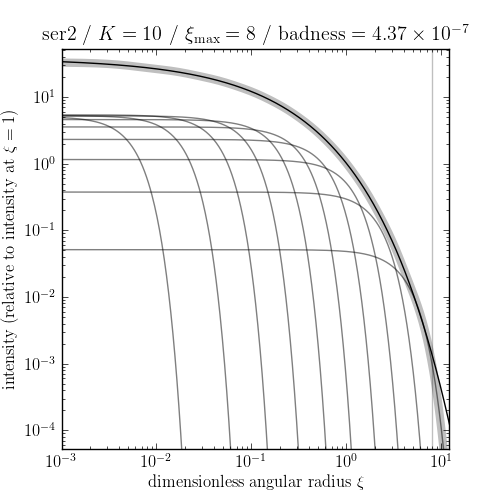
\includegraphics[width=\figurewidth]{ser2_K10_MR08_profile_log.png}%
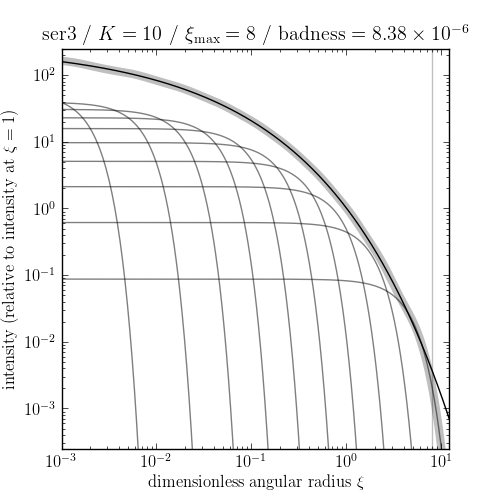
\includegraphics[width=\figurewidth]{ser3_K10_MR08_profile_log.png}\\
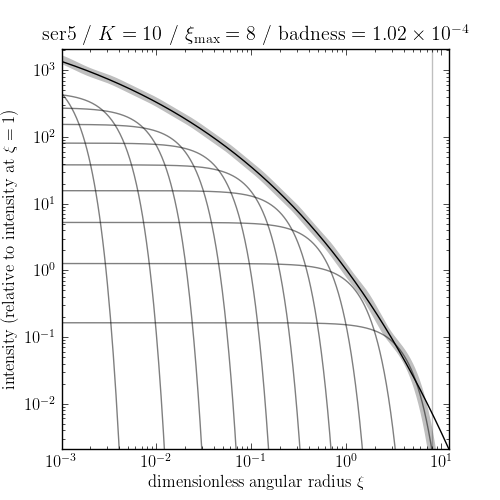
\includegraphics[width=\figurewidth]{ser5_K10_MR08_profile_log.png}%
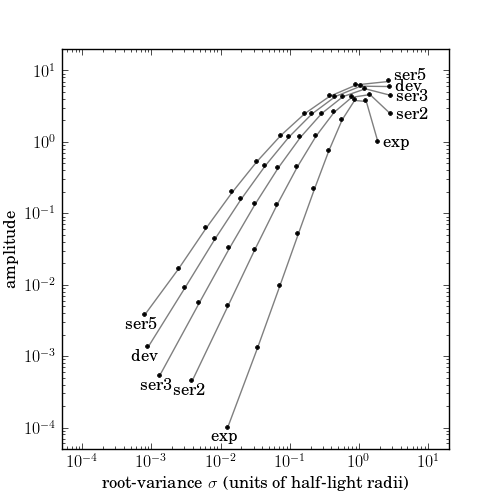
\includegraphics[width=\figurewidth]{mixtures_vs_model_K10.png}
\caption{Three ser profiles---with $n=2$, $3$, and $5$---and
  approximations.  The top-left, top-right, and bottom-left panels are
  equivalent to those in the top-right of \figurename~\ref{fig:exp}.
  \textsl{bottom-right:} The dependence on the amplitudes $a^{\ser}_m$
  and root-variances $\sqrt{v^{\ser}_m}$ on ser index $n$.}
\end{figure}

\clearpage
\begin{figure}
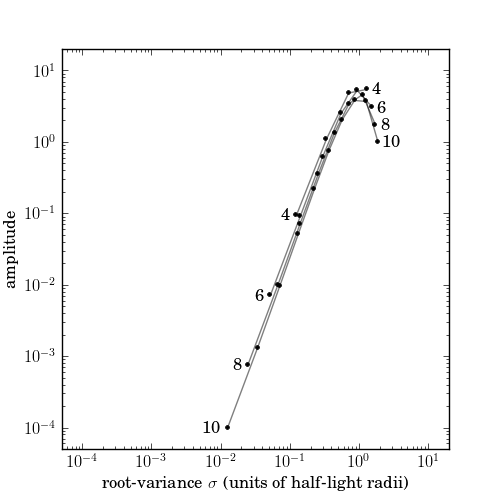
\includegraphics[width=\figurewidth]{mixtures_vs_K_exp.png}%
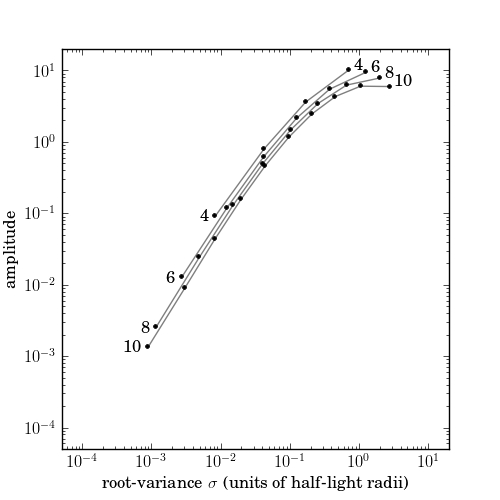
\includegraphics[width=\figurewidth]{mixtures_vs_K_dev.png}\\
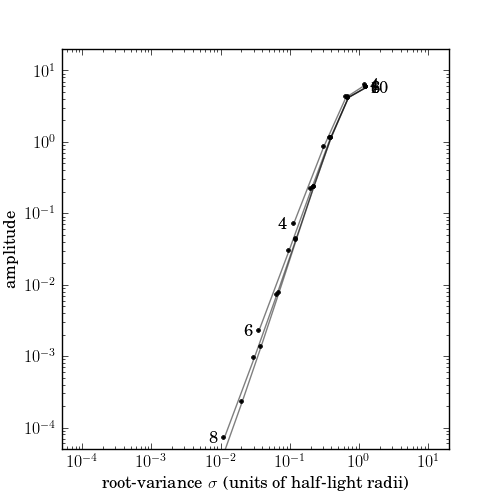
\includegraphics[width=\figurewidth]{mixtures_vs_K_lux.png}%
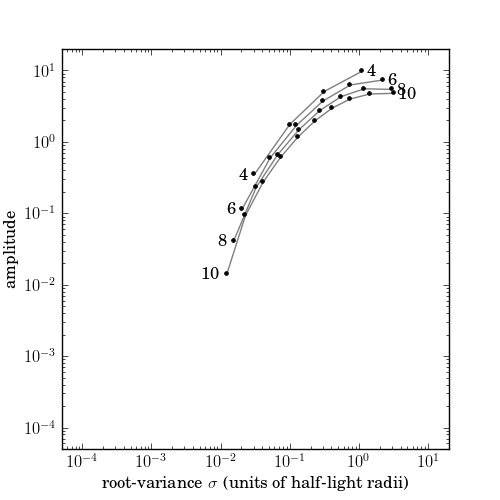
\includegraphics[width=\figurewidth]{mixtures_vs_K_luv.png}
\caption{Comparisons of approximations.  \textsl{top-left:} The
  dependence of amplitude $a^{\exp}_m$ and root-variance
  $\sqrt{v^{\exp}_m}$ on $M^{\exp}$ for the exp profile.
  \textsl{top-right:} The same but for the dev profile.
  \textsl{bottom-left:} The same but for the lux profile.
  \textsl{bottom-right:} The same but for the luv profile.}
\end{figure}

\end{document}
